\chapter{Implementacija i korisničko sučelje}
		
		
		\section{Korištene tehnologije i alati}
		
			\textbf{\textit{dio 2. revizije}}
			
			 \textit{Detaljno navesti sve tehnologije i alate koji su primijenjeni pri izradi dokumentacije i aplikacije. Ukratko ih opisati, te navesti njihovo značenje i mjesto primjene. Za svaki navedeni alat i tehnologiju je potrebno \textbf{navesti internet poveznicu} gdje se mogu preuzeti ili više saznati o njima}.
			
			
			\eject 
		
	
		\section{Ispitivanje programskog rješenja}
			
			\textbf{\textit{dio 2. revizije}}\\
			
			 \textit{U ovom poglavlju je potrebno opisati provedbu ispitivanja implementiranih funkcionalnosti na razini komponenti i na razini cijelog sustava s prikazom odabranih ispitnih slučajeva. Studenti trebaju ispitati temeljnu funkcionalnost i rubne uvjete.}
	
			
			\subsection{Ispitivanje komponenti}
			\text{Ispitivanje komponenti provedeno je koristeći Node.js frameworkove Mocha i Chai }
			
			\begin{figure}[hp]
                    \centering
                    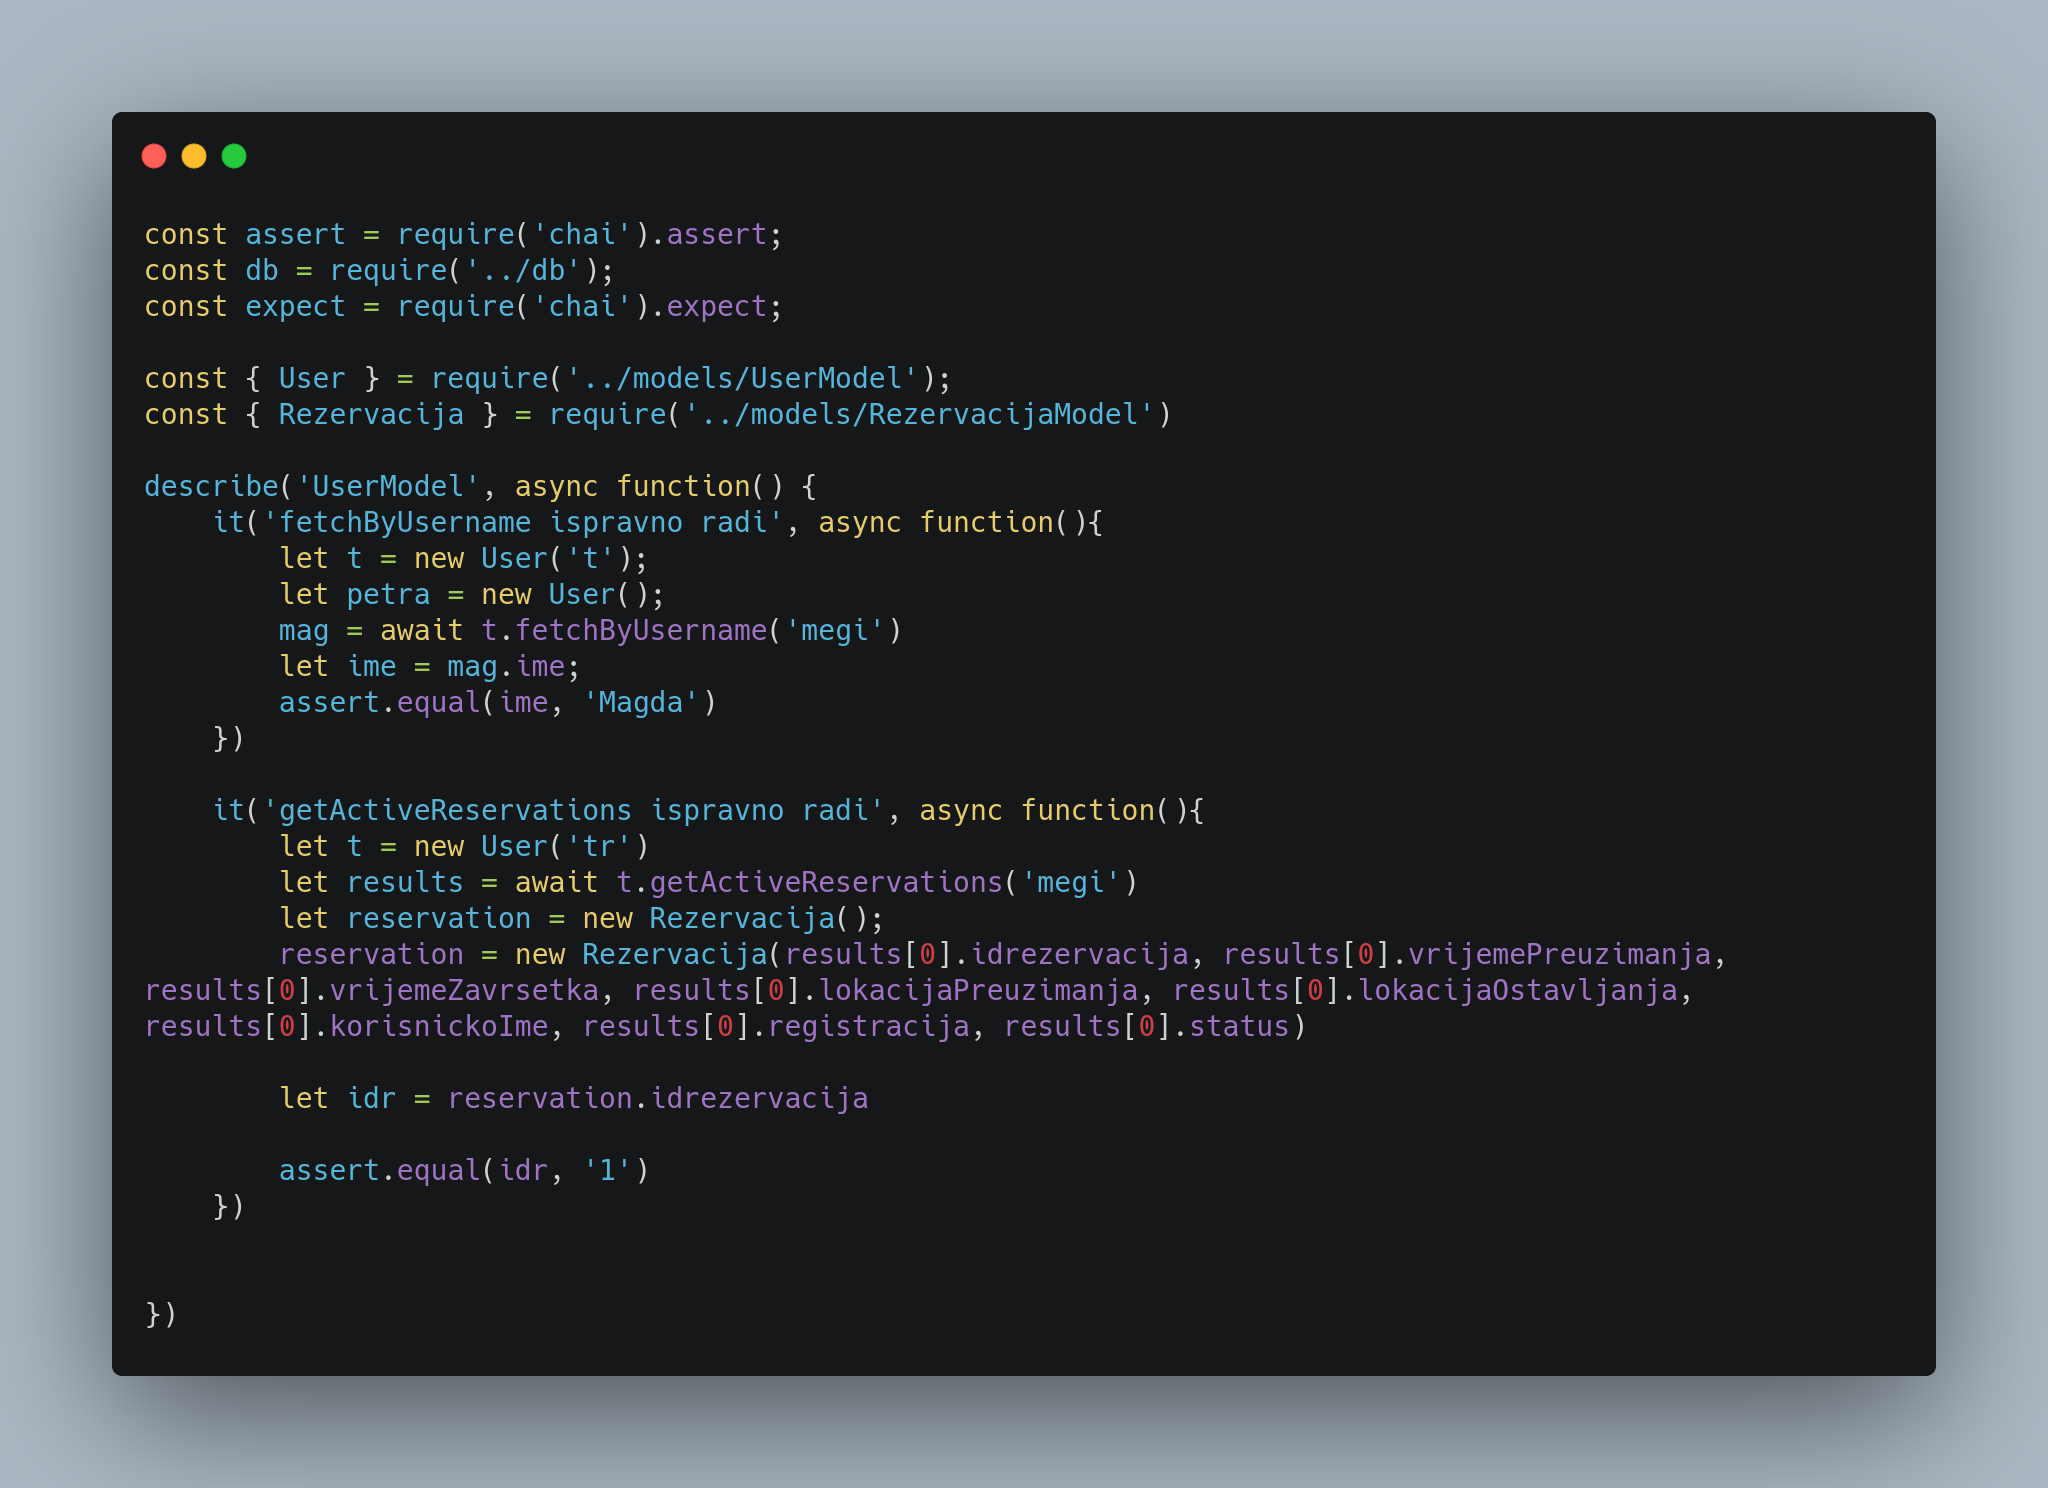
\includegraphics[width=15cm]{slike/UserModel.png}
                    \caption{Testiranje UserModela}
                    \label{fig:useCase-2}
                \end{figure}
			\eject 
			
	
			
			\begin{figure}[hp]
                    \centering
                    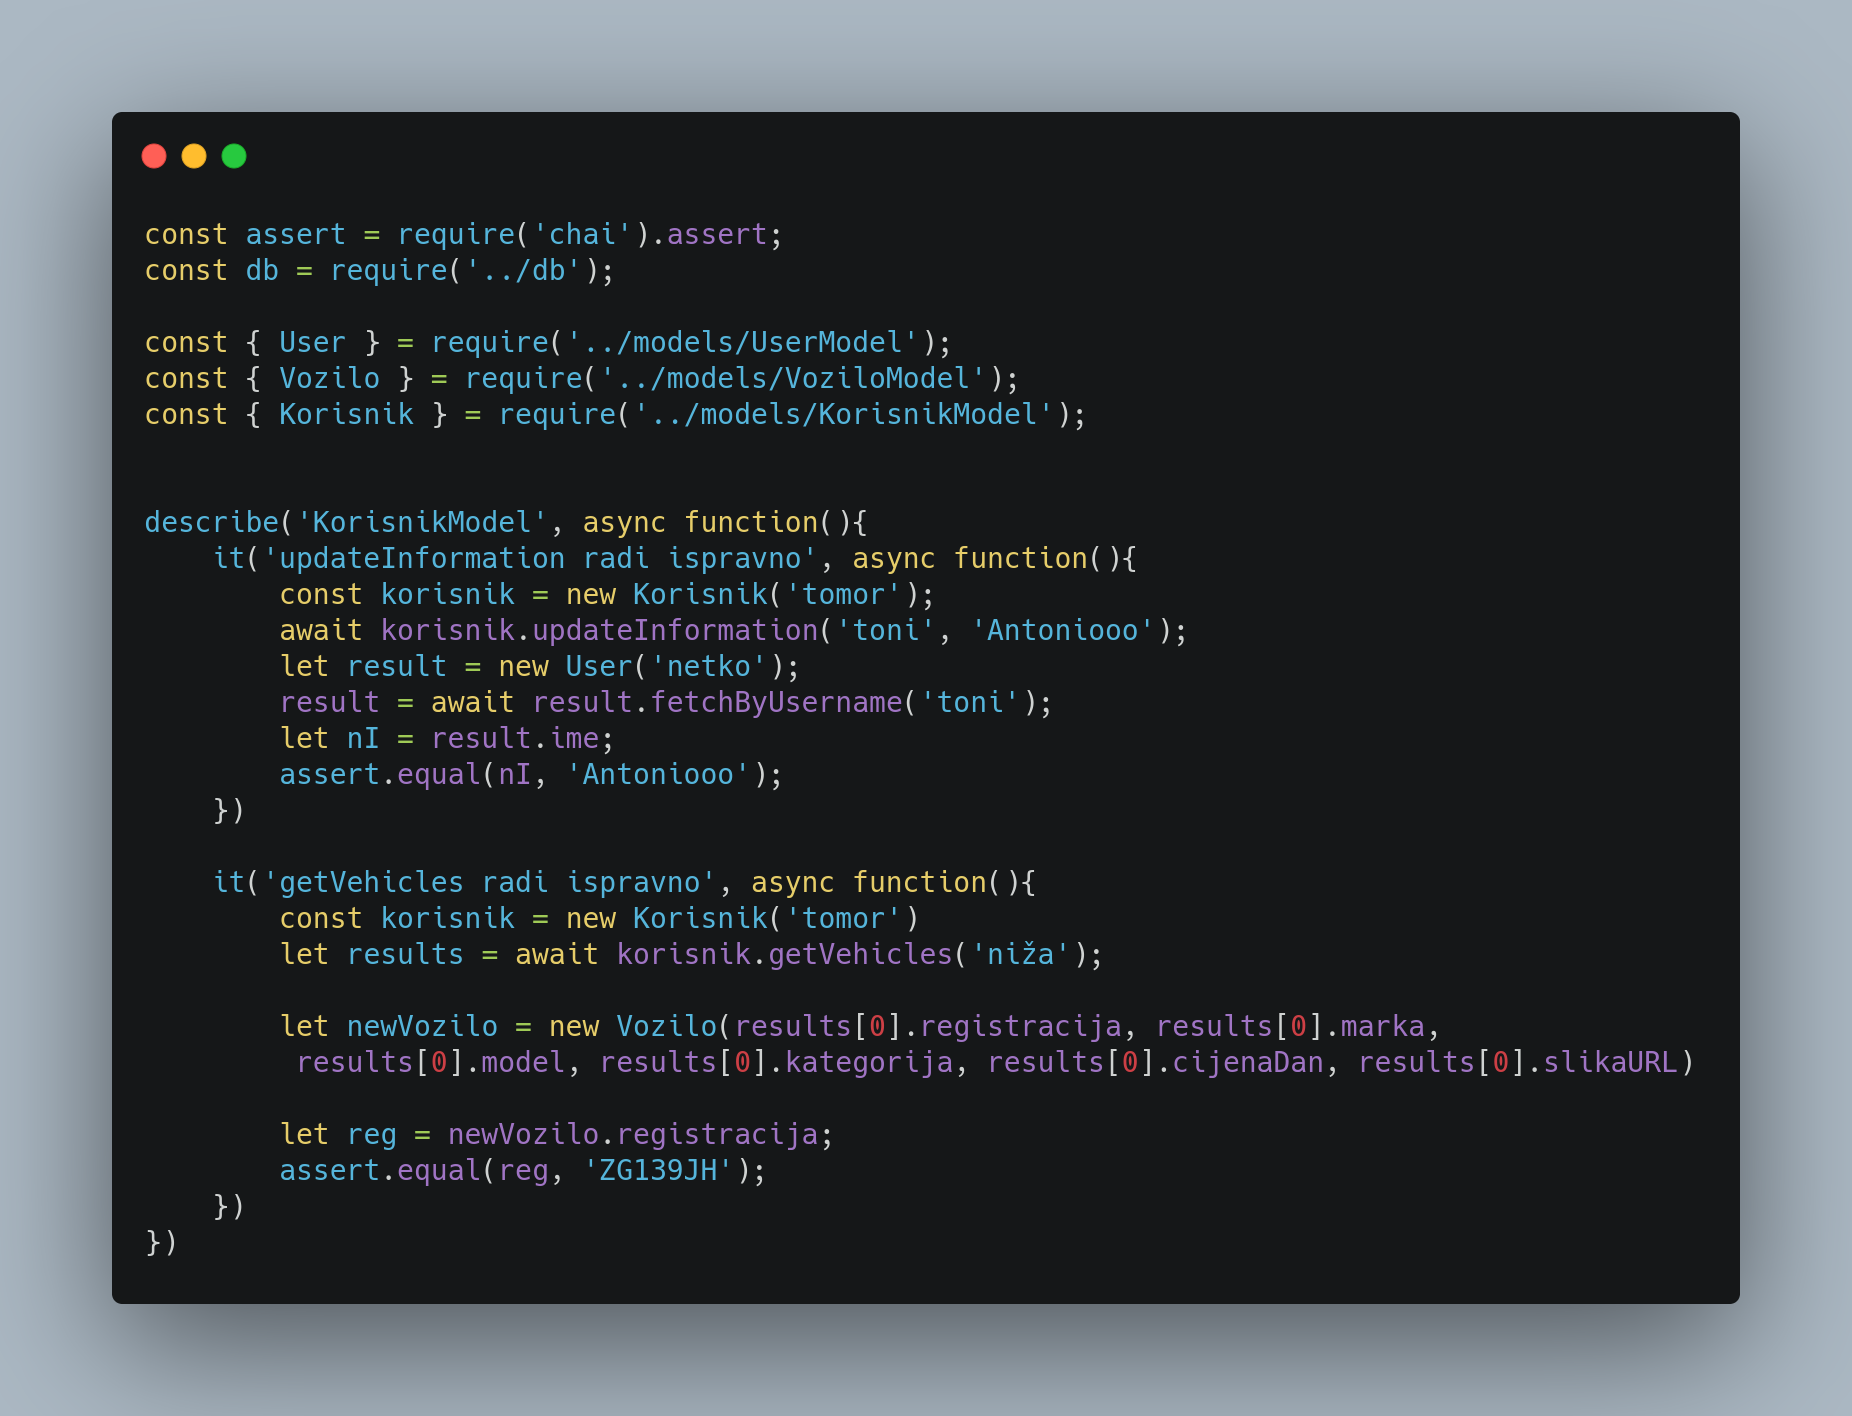
\includegraphics[width=15cm]{slike/KorisnikModel.png}
                    \caption{Testiranje KorisnikModela}
                    \label{fig:useCase-2}
                \end{figure}
			\eject 
			
			\begin{figure}[hp]
                    \centering
                    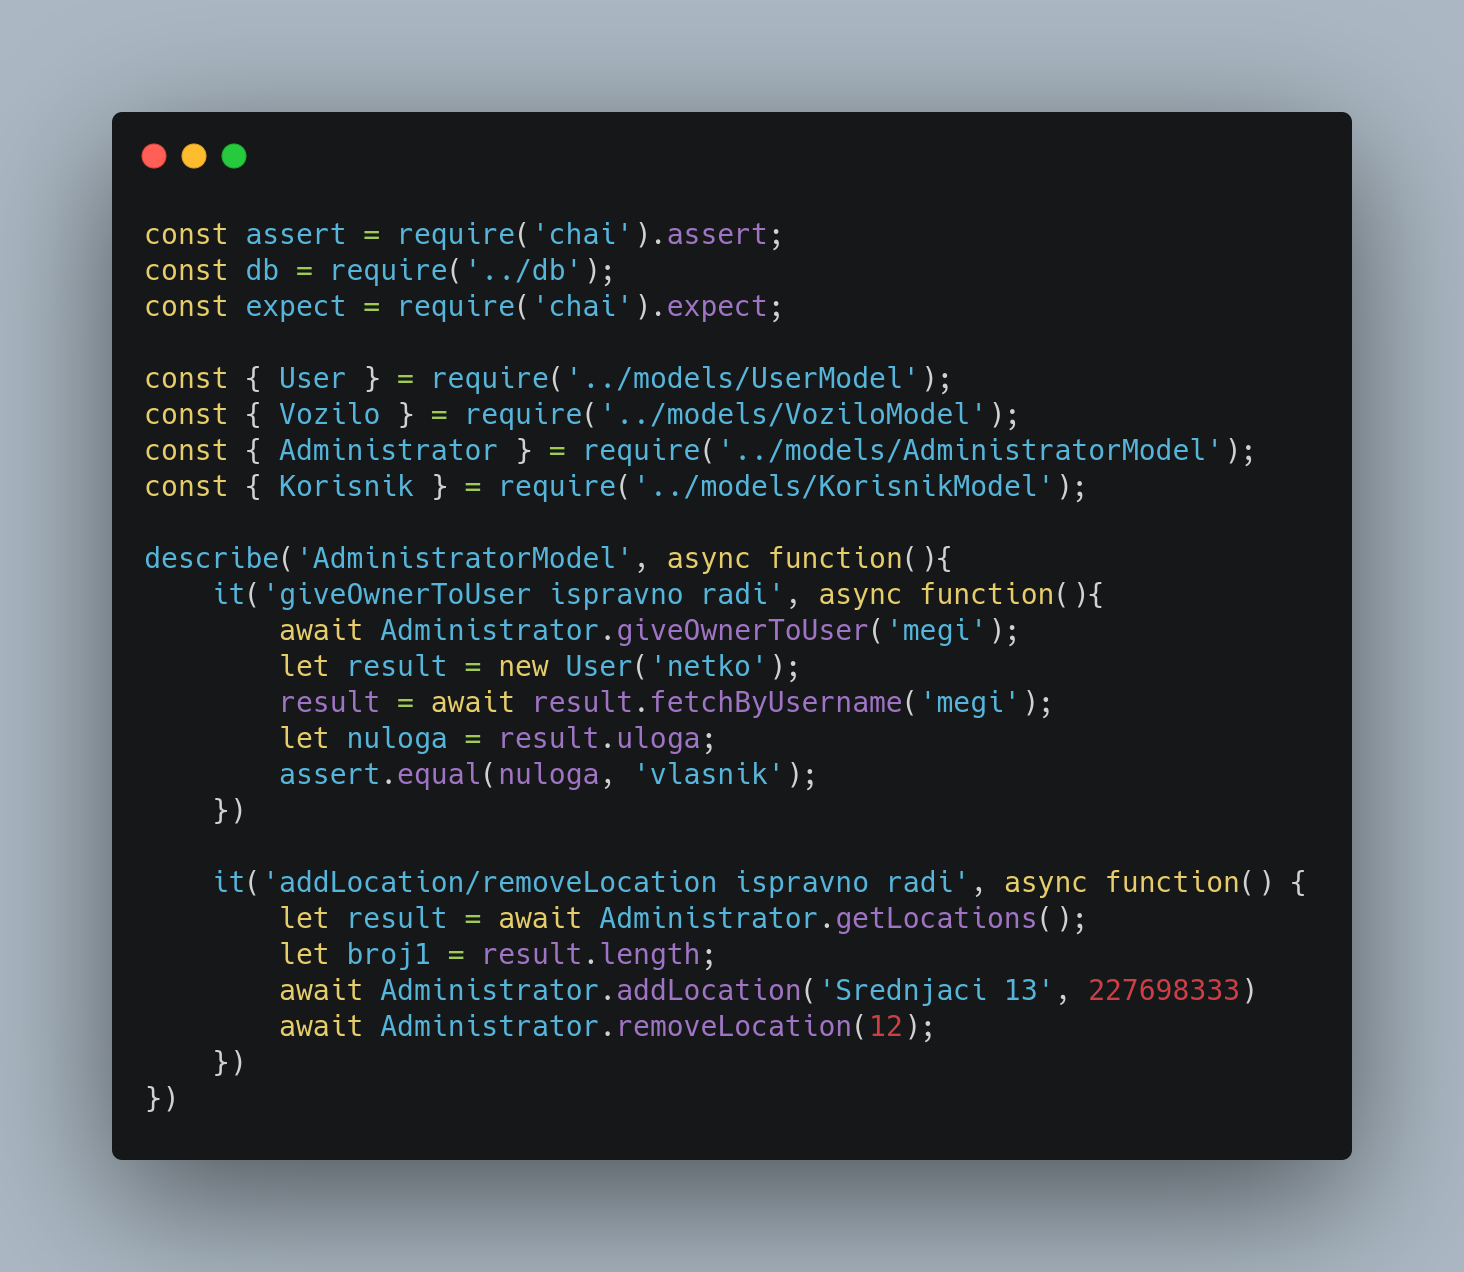
\includegraphics[width=15cm]{slike/AdministratorModel.png}
                    \caption{Testiranje AdministratorModela}
                    \label{fig:useCase-2}
                \end{figure}
			\eject 
			
			
			\begin{figure}[hp]
                    \centering
                    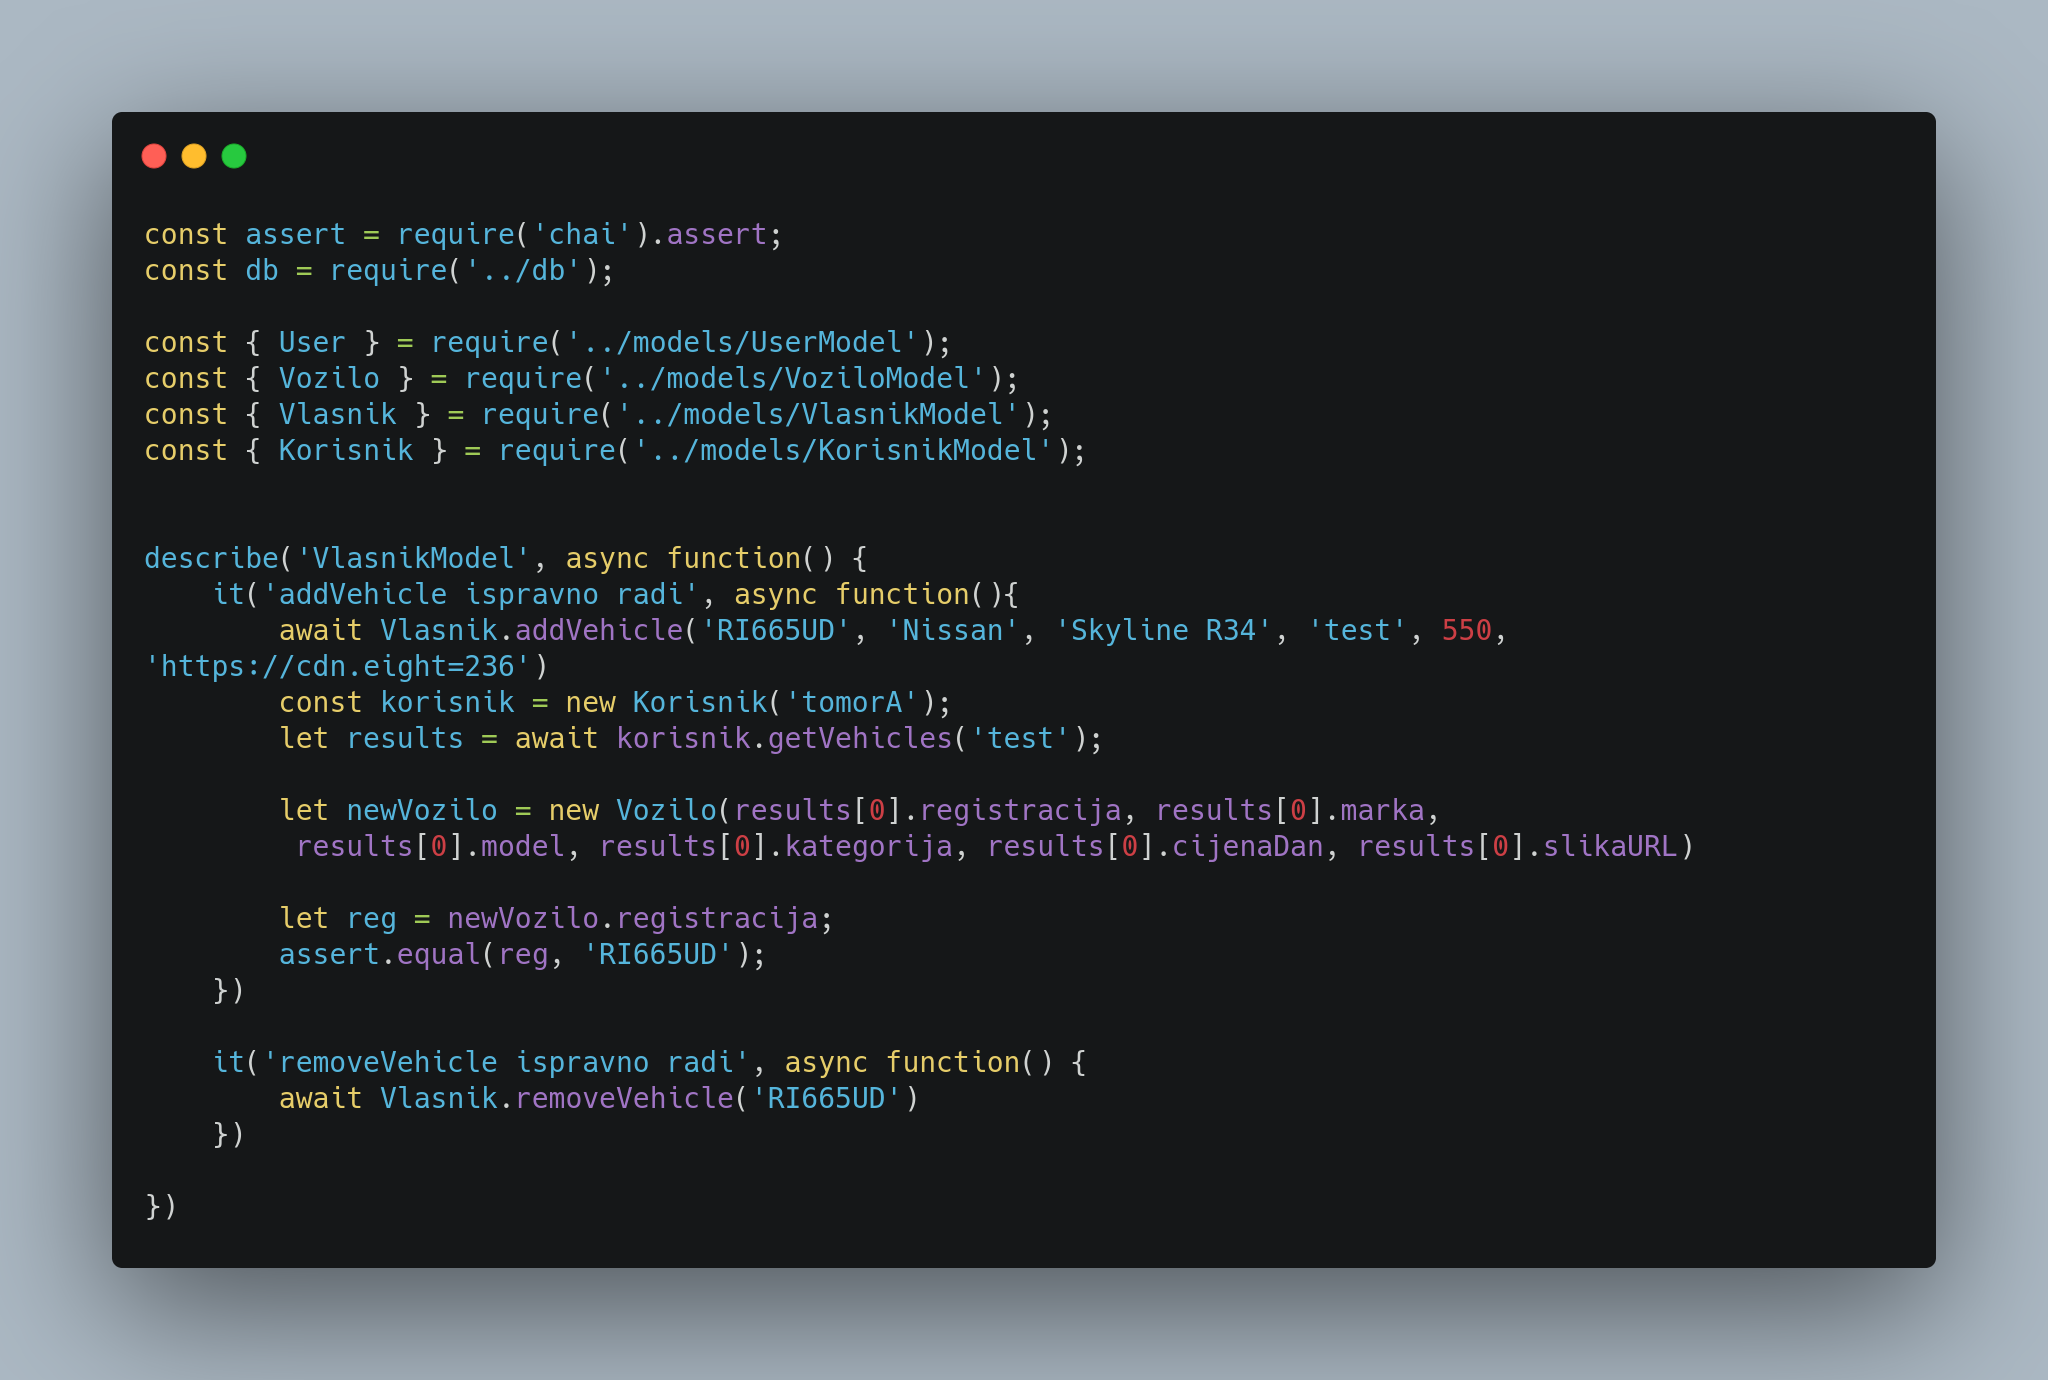
\includegraphics[width=15cm]{slike/VlasnikModel.png}
                    \caption{Testiranje VlasnikModela}
                    \label{fig:useCase-2}
                \end{figure}
			\eject 
			
			\begin{figure}[hp]
                    \centering
                    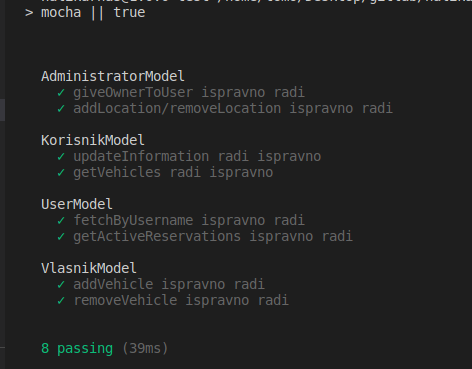
\includegraphics[width=15cm]{slike/rjesenjeeeee.png}
                    \caption{Rezultati testova}
                    \label{fig:useCase-2}
                \end{figure}
			\eject 
			
			
			
			\subsection{Ispitivanje sustava}
			    
			    \noindent{Ispitivanje sustava proveli smo koristeći Selenium WebDriver (\textit{https://selenium.dev/documentation/en/selenium-installation/}) unutar JUnit testova. Kodovi za ispitivanje ispravne i neisprave prijave dani su na slikama 5.6 i 5.7, a rezultati testa vidljivi su na slici 5.8.}
			
			\begin{figure}[hp]
                    \centering
                    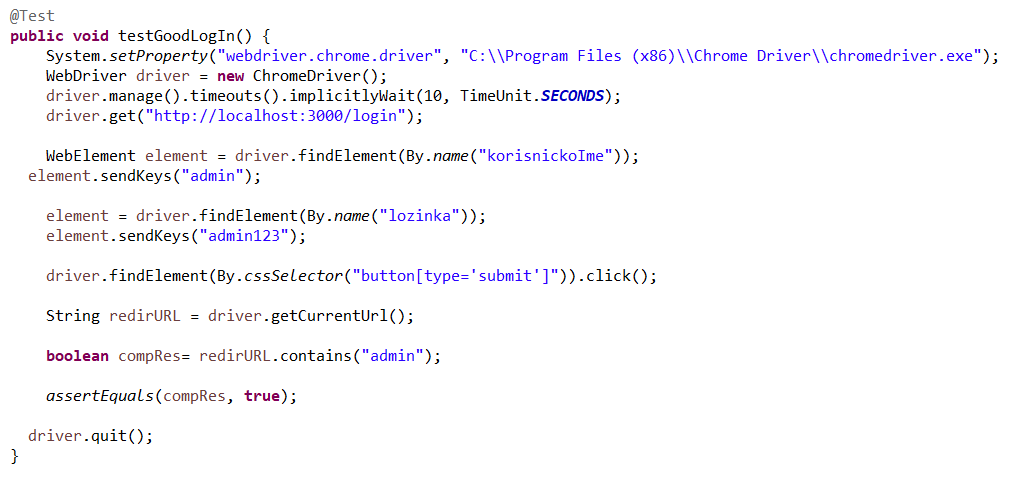
\includegraphics[width=15cm]{slike/koddobraprijava.png}
                    \caption{Kod ispravne prijave}
                    \label{fig:useCase-2}
                \end{figure}
			\eject
            
            \begin{figure}[hp]
                    \centering
                    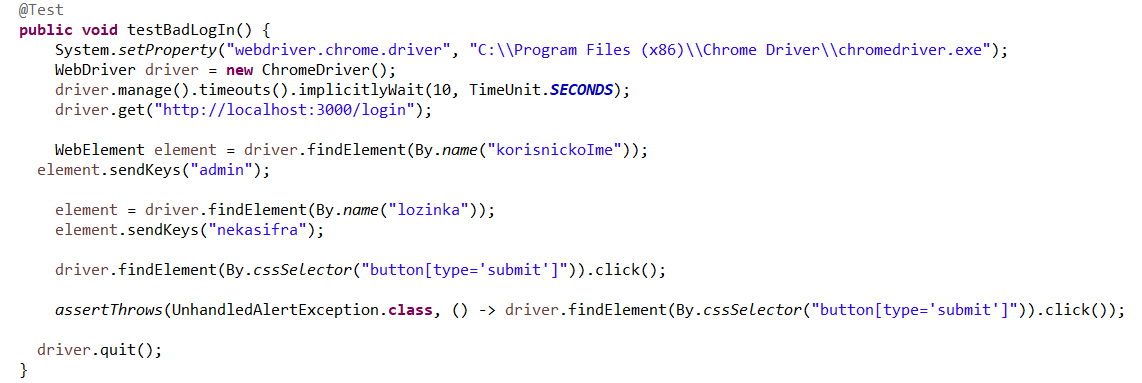
\includegraphics[width=15cm]{slike/kodlosaprijava.png}
                    \caption{Kod neispravne prijave}
                    \label{fig:useCase-2}
                \end{figure}
			\eject
			
			\begin{figure}[hp]
                    \centering
                    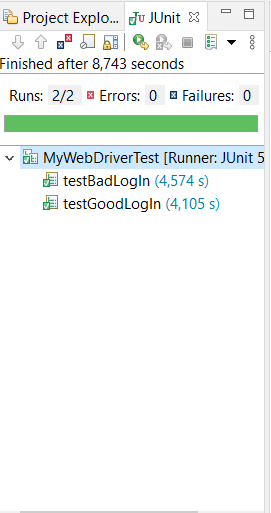
\includegraphics[width=15cm]{slike/logintests.png}
                    \caption{Rezultati testova}
                    \label{fig:useCase-2}
                \end{figure}
			\eject
			
			    \noindent{Kodovi za ispitivanje ispravne i neisprave pretrage vozila dani su na slikama 5.9 i 5.10, a rezultati testa vidljivi su na slici 5.11. Kod dobre pretrage nakon unosa datuma, klikom na gumb prikazuju nam se auti koji se mogu rezervirati. U slučaju unosa neispravnog datuma, stranica nas o tom obavještava pomoću alert box-a.}
			
			\begin{figure}[hp]
                    \centering
                    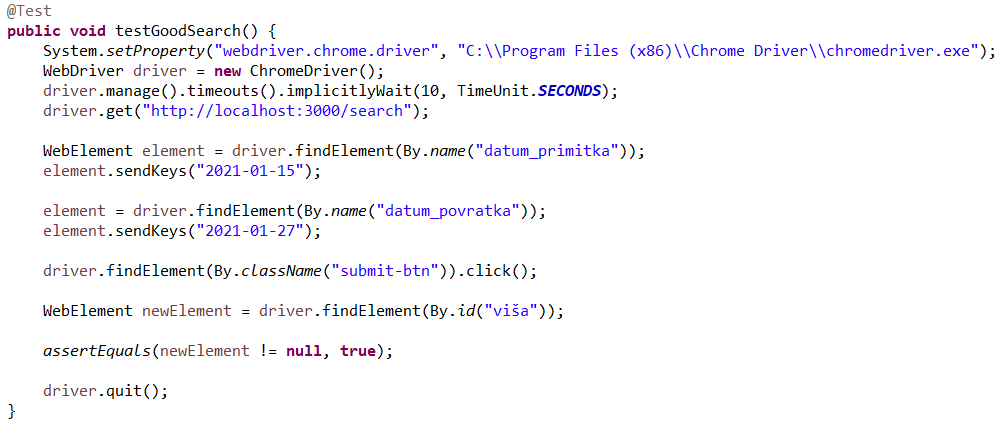
\includegraphics[width=15cm]{slike/koddobrapretraga.png}
                    \caption{Kod ispravne pretrage}
                    \label{fig:useCase-2}
                \end{figure}
			\eject
			
			\begin{figure}[hp]
                    \centering
                    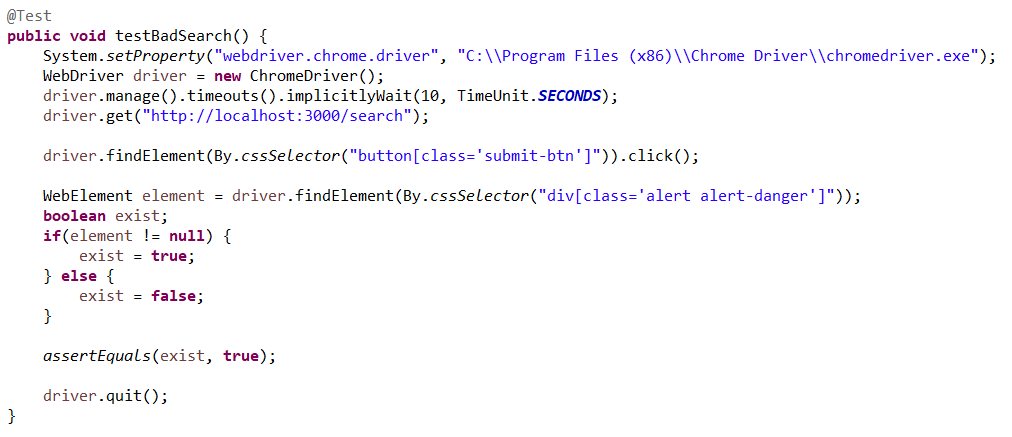
\includegraphics[width=15cm]{slike/kodlosapretraga.png}
                    \caption{Kod neispravne pretrage}
                    \label{fig:useCase-2}
                \end{figure}
			\eject
			
			\begin{figure}[hp]
                    \centering
                    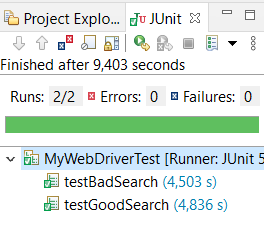
\includegraphics[width=15cm]{slike/searchtests.png}
                    \caption{Rezultati testova}
                    \label{fig:useCase-2}
                \end{figure}
			\eject
			
			\noindent{Kodovi za ispitivanje uspješne i neuspješne lozinke dani su na slikama 5.12 i 5.13, a rezultati testova dani su na slikama 5.14 i 5.15. U slučaju uspješne promjene lozinke, korisnik se preusmjerava na početnu stranicu, dok u slučaju neuspješne promjene korisnik dobije poruku o neuspjehu.}
			
			\begin{figure}[hp]
                    \centering
                    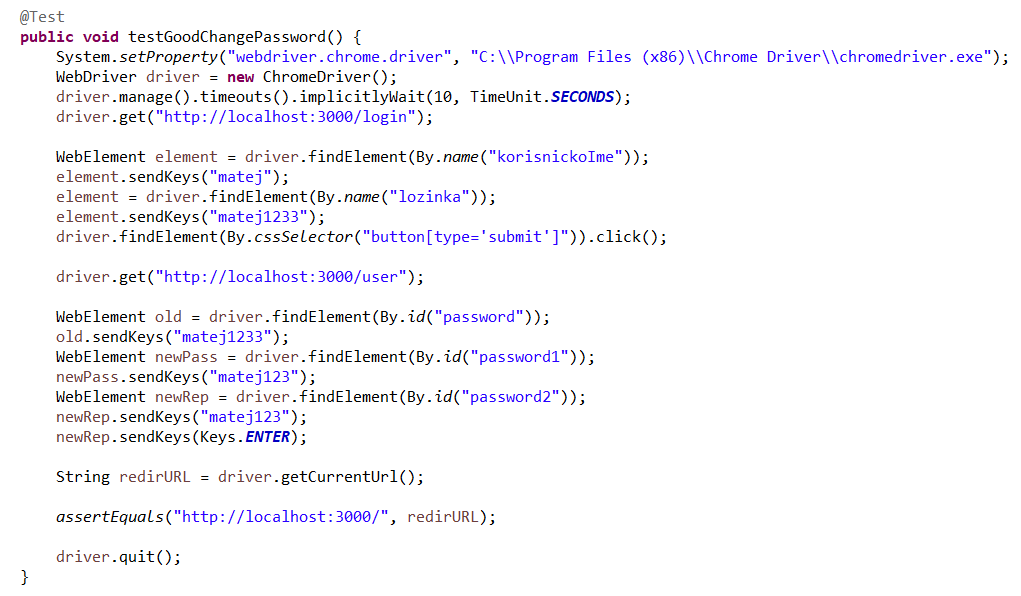
\includegraphics[width=15cm]{slike/koddobrapromjenalozinke.png}
                    \caption{Uspješna promjena lozinke}
                    \label{fig:useCase-2}
                \end{figure}
			\eject
			
			\begin{figure}[hp]
                    \centering
                    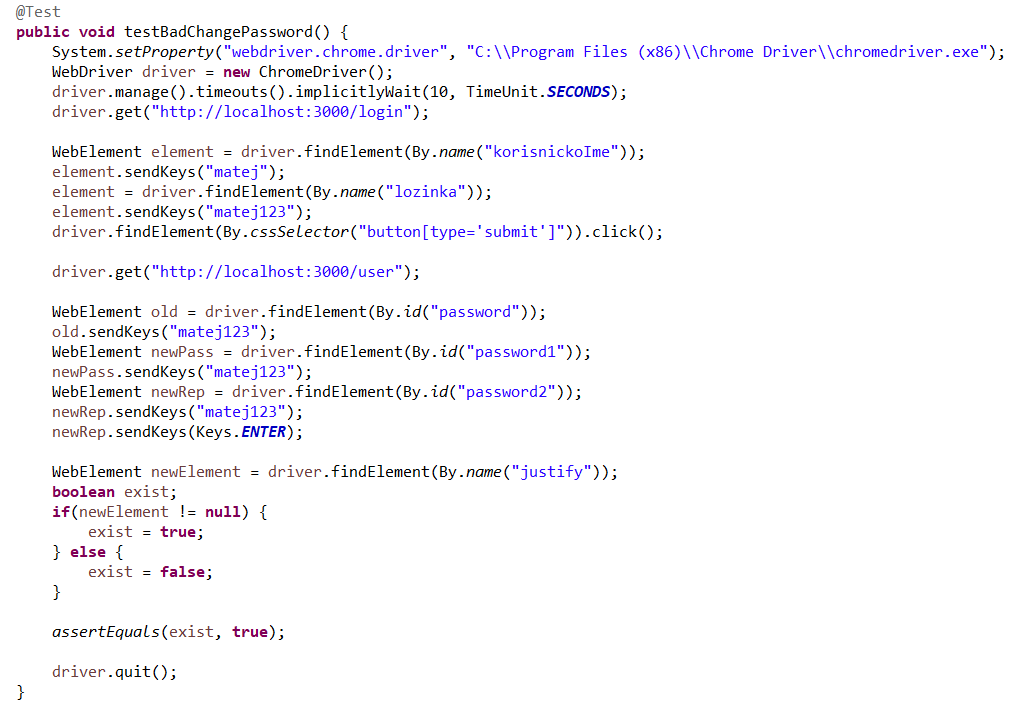
\includegraphics[width=15cm]{slike/kodlosapromjenalozinke.png}
                    \caption{Neuspješna promjena lozinke}
                    \label{fig:useCase-2}
                \end{figure}
			\eject
			
			\begin{figure}[hp]
                    \centering
                    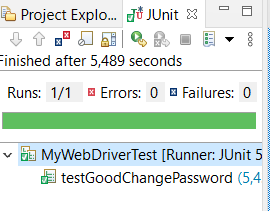
\includegraphics[width=15cm]{slike/passwordgood.png}
                    \caption{Rezultat testa uspješne promjene lozinke}
                    \label{fig:useCase-2}
                \end{figure}
			\eject
			
			\begin{figure}[hp]
                    \centering
                    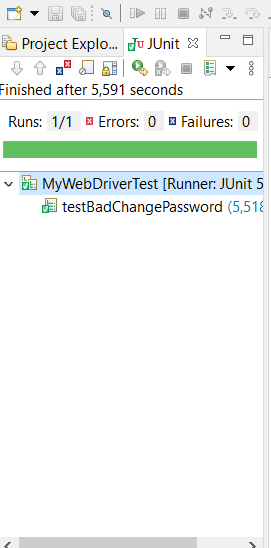
\includegraphics[width=15cm]{slike/passwordbad.png}
                    \caption{Rezultat testa neuspješne promjene lozinke}
                    \label{fig:useCase-2}
                \end{figure}
			\eject
			
			\noindent{Kodovi za ispitivanje rezervacije vozila dani su na slikama 5.16 i 5.17, a rezultati testova dani su na slikama 5.18 i 5.19. Prijavljeni korisnik može rezervirati auto, dok neprijavljeni korisnik ne može zato što mu gumb za rezervaciju nije vidljiv.}
			
			\begin{figure}[hp]
                    \centering
                    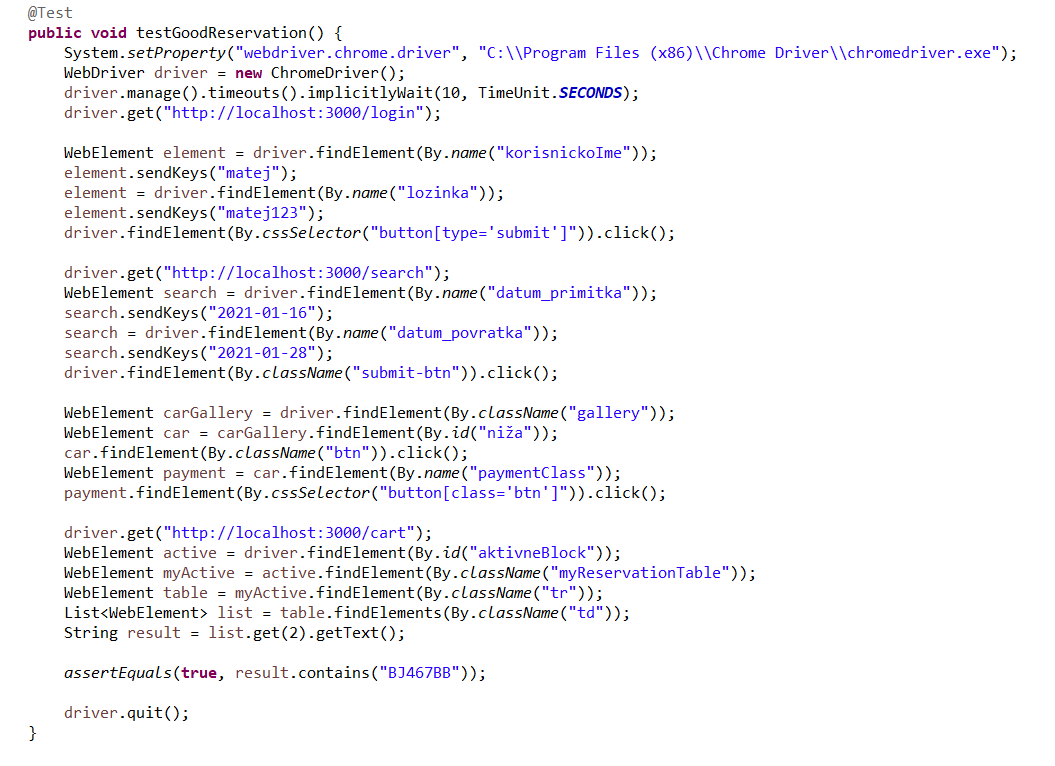
\includegraphics[width=15cm]{slike/koddobrarezervacija.png}
                    \caption{Uspješna rezervacija}
                    \label{fig:useCase-2}
                \end{figure}
			\eject
			
			\begin{figure}[hp]
                    \centering
                    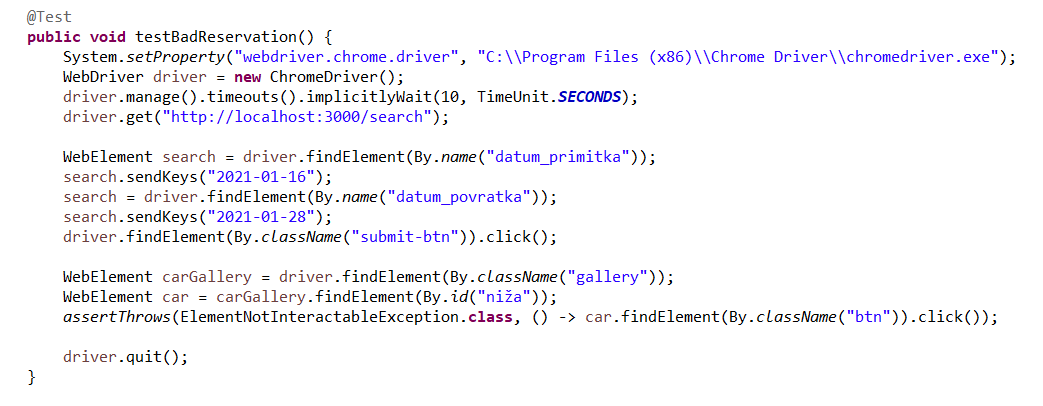
\includegraphics[width=15cm]{slike/kodlosarezervacija.png}
                    \caption{Neuspješna rezervacija}
                    \label{fig:useCase-2}
                \end{figure}
			\eject
			
			\begin{figure}[hp]
                    \centering
                    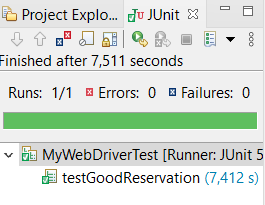
\includegraphics[width=15cm]{slike/reservationgood.png}
                    \caption{Rezultat testa uspješne rezervacije}
                    \label{fig:useCase-2}
                \end{figure}
			\eject
			
			\begin{figure}[hp]
                    \centering
                    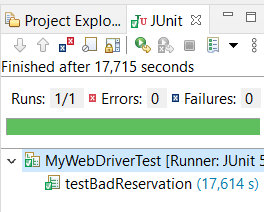
\includegraphics[width=15cm]{slike/reservationbad.png}
                    \caption{Rezultat testa neuspješne rezervacije}
                    \label{fig:useCase-2}
                \end{figure}
			\eject
			
			\eject 
		
		
		\section{Dijagram razmještaja}
			
			
			
			  \noindent Dijagram razmještaja prikazuje radno okruženje sklopovlja i programske potpore. Na poslužiteljskom računalu se nalazi poslužitelj za bazu podataka i web poslužitelj. Na klijentskom računalu koristi se web preglednik kako bi se pristupilo web alikaciji. Komunikacija između računala korisnika i poslužitelja odvija se preko HTTP veze.
			
			\begin{figure}[hp]
                    \centering
                    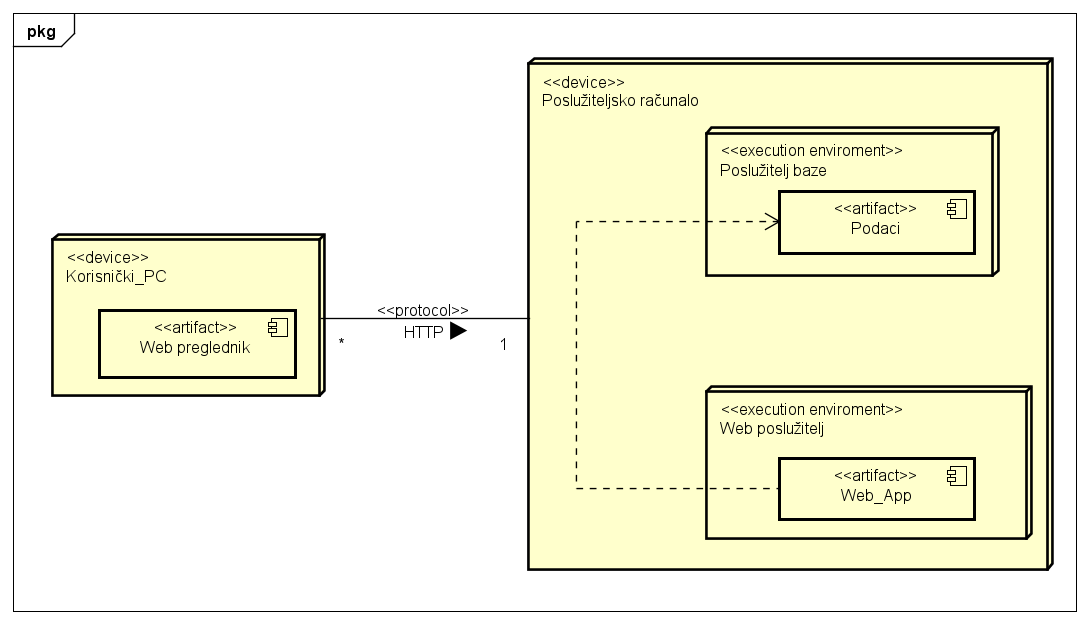
\includegraphics[width=16cm]{slike/Dijagram_razmjestaja.png}
                    \caption{Dijagram razmještaja}
                    \label{fig:DR_01}
                \end{figure}
			    
			\eject 
			
		
		\section{Upute za puštanje u pogon}
		
			\textbf{\textit{dio 2. revizije}}\\
		
			 \textit{U ovom poglavlju potrebno je dati upute za puštanje u pogon (engl. deployment) ostvarene aplikacije. Na primjer, za web aplikacije, opisati postupak kojim se od izvornog kôda dolazi do potpuno postavljene baze podataka i poslužitelja koji odgovara na upite korisnika. Za mobilnu aplikaciju, postupak kojim se aplikacija izgradi, te postavi na neku od trgovina. Za stolnu (engl. desktop) aplikaciju, postupak kojim se aplikacija instalira na računalo. Ukoliko mobilne i stolne aplikacije komuniciraju s poslužiteljem i/ili bazom podataka, opisati i postupak njihovog postavljanja. Pri izradi uputa preporučuje se \textbf{naglasiti korake instalacije uporabom natuknica} te koristiti što je više moguće \textbf{slike ekrana} (engl. screenshots) kako bi upute bile jasne i jednostavne za slijediti.}
			
			
			 \textit{Dovršenu aplikaciju potrebno je pokrenuti na javno dostupnom poslužitelju. Studentima se preporuča korištenje neke od sljedećih besplatnih usluga: \href{https://aws.amazon.com/}{Amazon AWS}, \href{https://azure.microsoft.com/en-us/}{Microsoft Azure} ili \href{https://www.heroku.com/}{Heroku}. Mobilne aplikacije trebaju biti objavljene na F-Droid, Google Play ili Amazon App trgovini.}
			
			
			\eject 
